
The objective of this problem is to design an observer that estimates the state of the system and uses the estimated state in the controller designed in Homework~\ref{ds:single_link_arm}.\ref{chap:state-feedback-integrator}.

\begin{description}\item[]
\item[(a)] The first step is to modify the Simulink diagram so that we can observe the performance of the observer.  Modify the Simulink diagram from Homework~\ref{ds:single_link_arm}.1\ref{chap:state-feedback-integrator} so that the output of the s-function defining the dynamics is both $y$ and $x$ as shown in Figure~\ref{fig:ss_hw_arm_18}.  In addition, modify the Simulink diagram so that the controller outputs both $u$ and $\hat{x}$, as also shown in Figure~\ref{fig:ss_hw_arm_18}.
\begin{figure}[hbt]
  \centering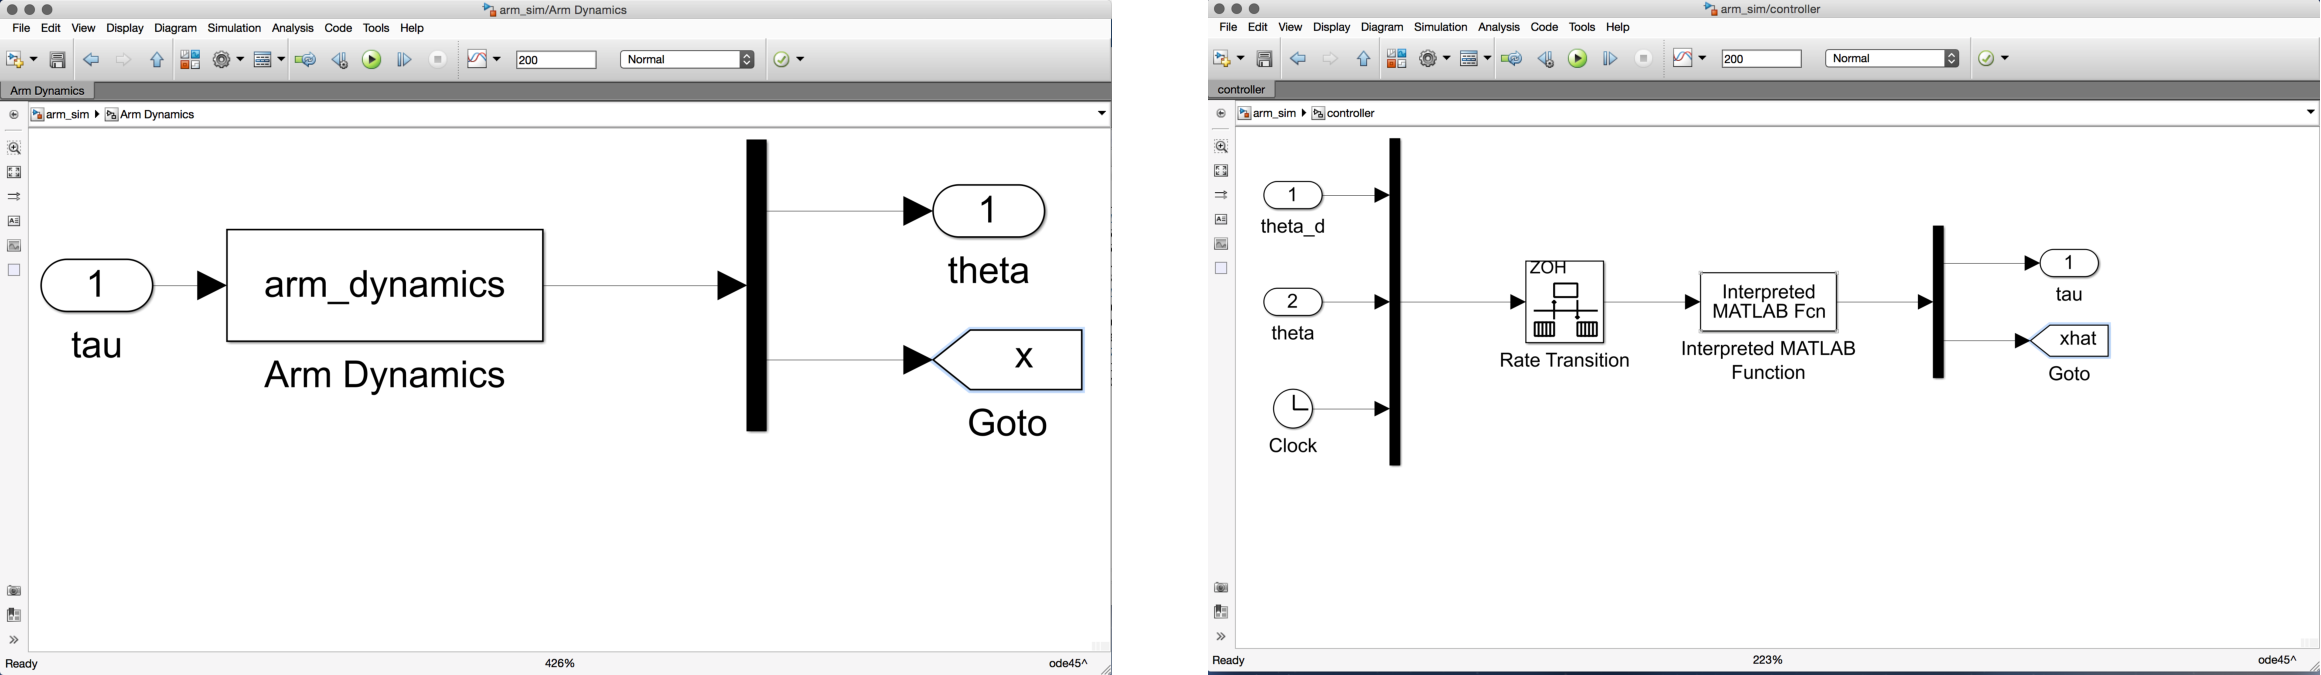
\includegraphics[width=0.95\textwidth]{4_observer_based/figures/ss_hw_arm_18}
  \caption{}
  \label{fig:ss_hw_arm_18}  
\end{figure}
The animation block can also be modified to include plots of $x$ and $\hat{x}$ and also the estimation error $x-\hat{x}$, as shown in Figure~\ref{fig:ss_hw_arm_18a}.
\begin{figure}[hbt]
  \centering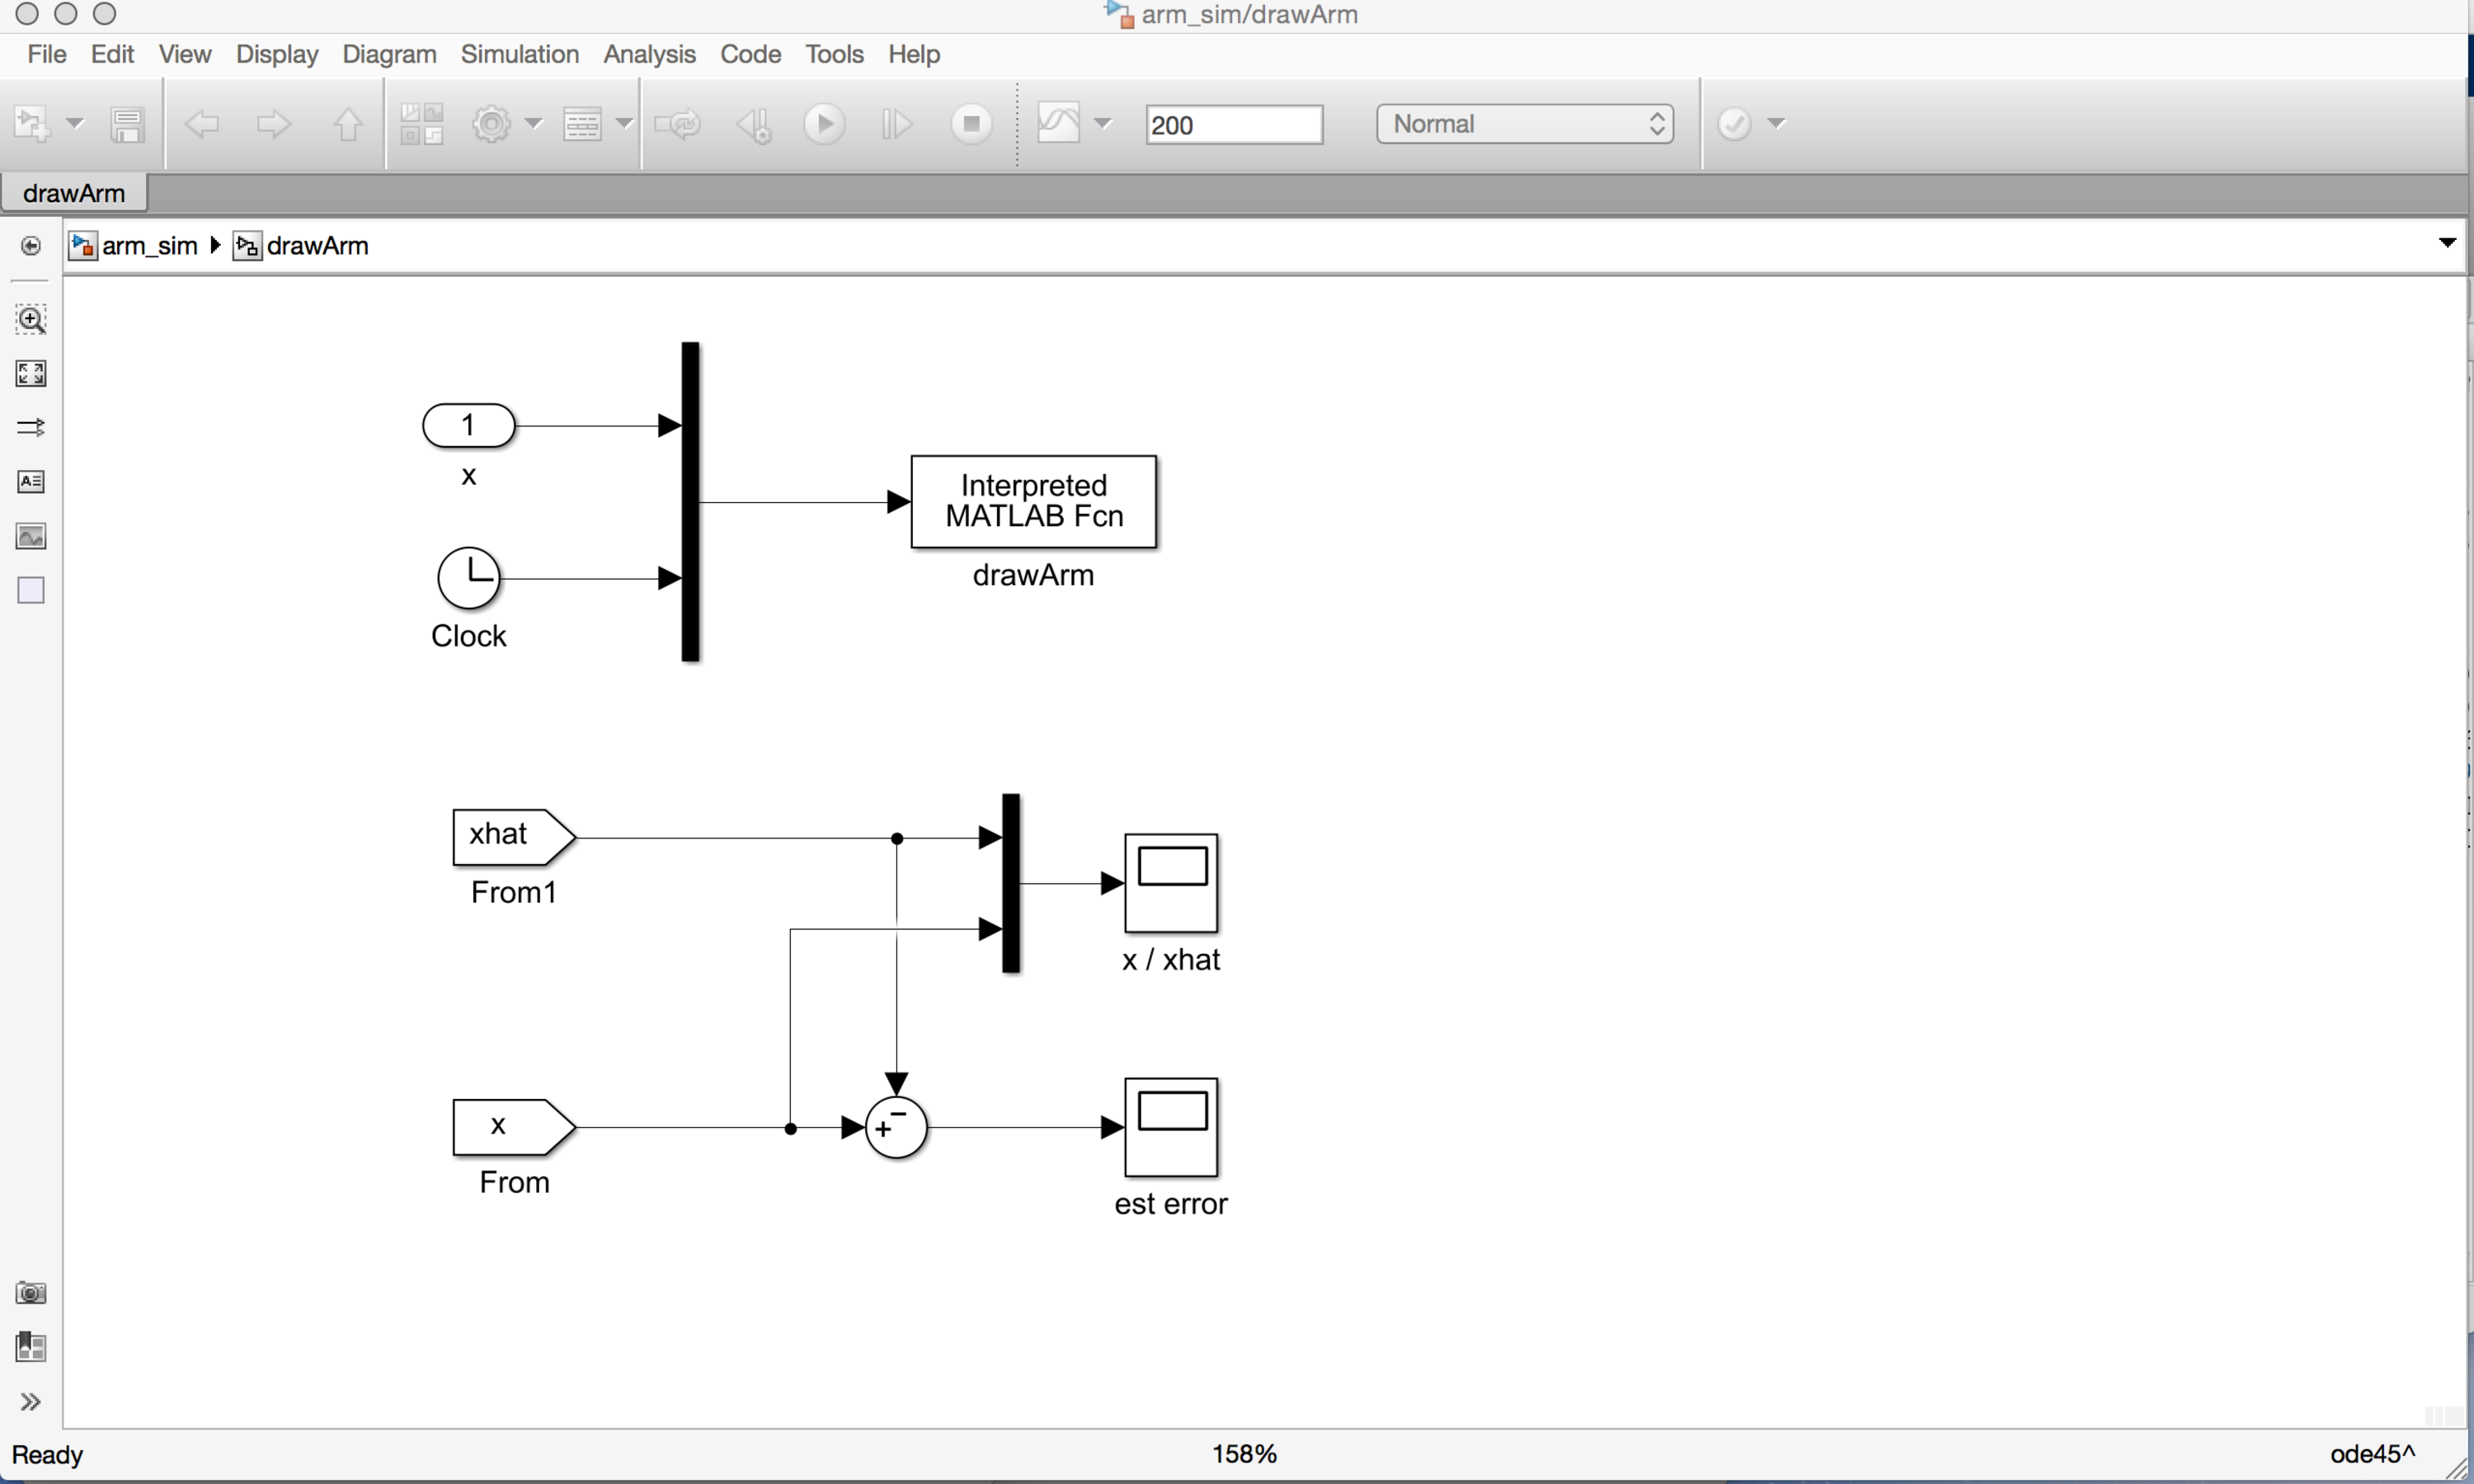
\includegraphics[width=0.95\textwidth]{4_observer_based/figures/ss_hw_arm_18a}
  \caption{}
  \label{fig:ss_hw_arm_18a}  
\end{figure}
The s-function defining the system will need to be modified so that the output of the block is both the normal output, as well as the actual state:
\begin{lstlisting}
sizes.NumOutputs     = 1+2; 

function sys=mdlOutputs(t,x,u,P)
  theta    = x(1);
  thetadot = x(2);
  tau      = u(1);
  sys = [theta; x];
\end{lstlisting}

Similarly, the output of the control block will need to be modified so that the output of the function is both the control output $u$ as well as the state estimate $\hat{x}$:
\begin{lstlisting}
function out=arm_ctrl(in,P)
	% control code goes here
    out = [u; xhat];   
end
\end{lstlisting}

\item[(b)] For the sake of understanding the function of the observer, for this problem we will use exact parameters, without an input disturbance.  Modify {\tt  arm\_dynamics.m} so that the parameters known to the controller are the actual plant parameters (uncertainty parameter $\alpha=0$).
\item[(c)] Verify that the state space system is observable by checking that $\text{rank}(\mathcal{O}_{A,C})=n$.
\item[(d)] In the control block, add an observer to estimate the state $\hat{x}$, and use the estimate of the state in your feedback controller.
Tune the poles of the controller and observer to obtain good performance.  
\item[(e)] As motivation for the next chapter, add an input disturbance to the system of $0.01$ and observe that there is steady state error in the response even though there is an integrator.  This is caused by a steady state error in the observation error.  In the next chapter we will show how to remove the steady state error in the observation error.
\end{description}
